\documentclass{standalone}
\usepackage{tikz}
\usetikzlibrary{patterns}
\usetikzlibrary{positioning}
\usetikzlibrary{patterns, positioning}
\usetikzlibrary{shapes.misc}
\usepackage[outline]{contour}
\contourlength{1.5pt} 
\usepackage[sfdefault]{ClearSans}

\begin{document}
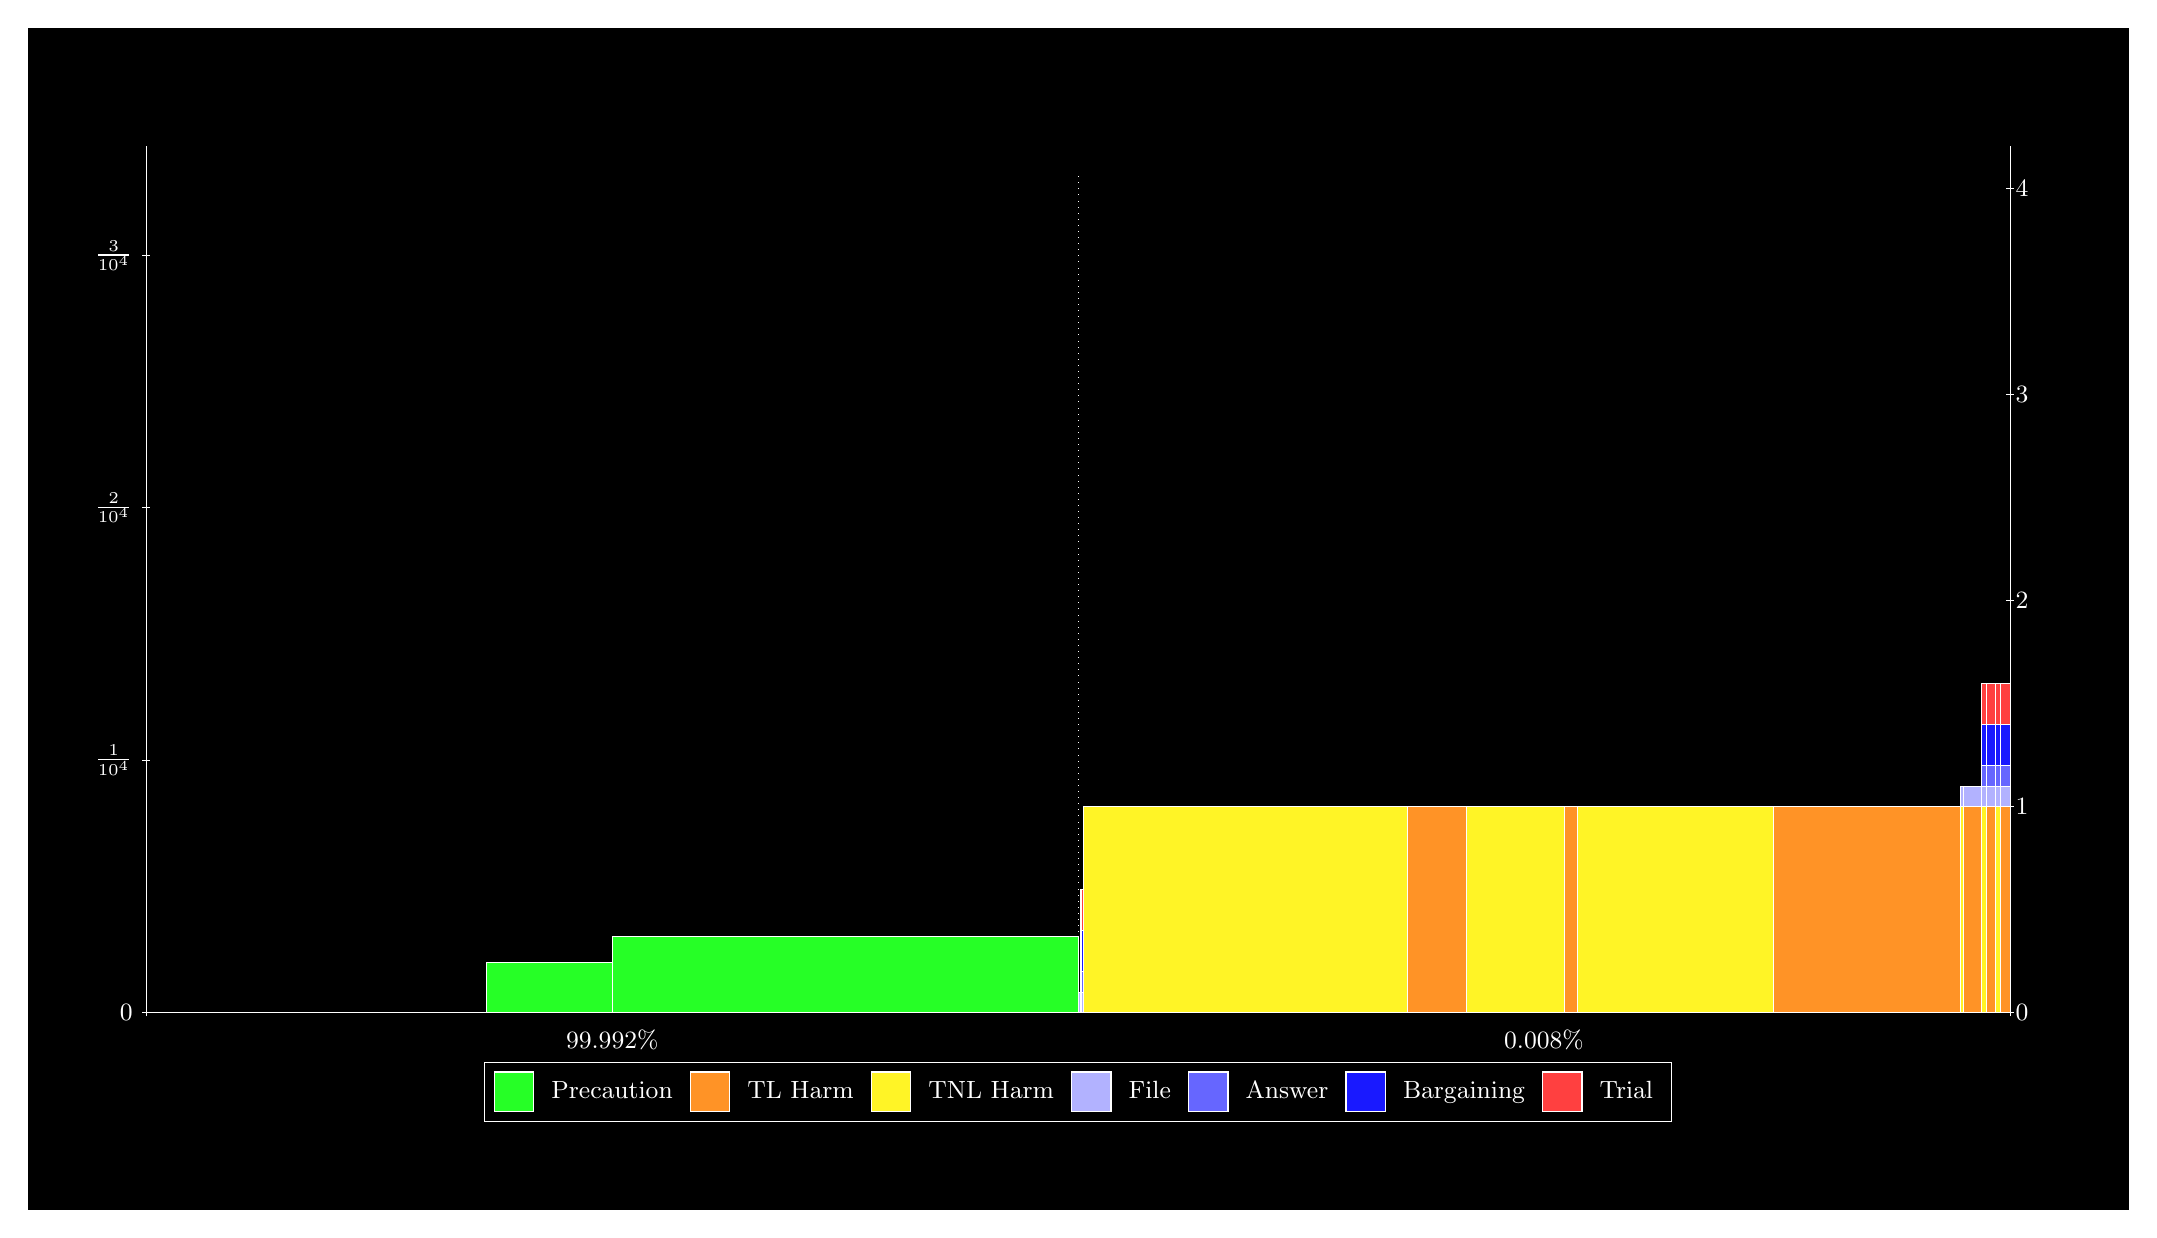
\begin{tikzpicture}
\draw[fill=black] (0,0) rectangle (26.667,15);
\draw[fill=green!85,draw=white,very thin] (5.8205,2.5) rectangle (7.4166,3.141);
\draw[fill=green!85,draw=white,very thin] (7.4166,2.5) rectangle (13.333,3.4616);
\draw[fill=blue!30,draw=white,very thin] (13.333,2.5) rectangle (13.359,2.7616);
\draw[fill=blue!30,draw=white,very thin] (13.359,2.5) rectangle (13.377,2.7616);
\draw[fill=blue!60,draw=white,very thin] (13.359,2.7616) rectangle (13.377,3.0231);
\draw[fill=blue!90,draw=white,very thin] (13.359,3.0231) rectangle (13.377,3.5463);
\draw[fill=red!75,draw=white,very thin] (13.359,3.5463) rectangle (13.377,4.0694);
\draw[fill=green!85,draw=white,very thin] (13.377,2.5) rectangle (13.401,2.5001);
\draw[fill=blue!30,draw=white,very thin] (13.377,2.5001) rectangle (13.401,2.7616);
\draw[fill=blue!60,draw=white,very thin] (13.377,2.7616) rectangle (13.401,3.0232);
\draw[fill=blue!90,draw=white,very thin] (13.377,3.0232) rectangle (13.401,3.5463);
\draw[fill=red!75,draw=white,very thin] (13.377,3.5463) rectangle (13.401,4.0695);
\draw[fill=yellow!85,draw=white,very thin] (13.401,2.5) rectangle (17.514,5.1157);
\draw[fill=orange!85,draw=white,very thin] (17.514,2.5) rectangle (18.264,5.1157);
\draw[fill=green!85,draw=white,very thin] (18.264,2.5) rectangle (19.508,2.5001);
\draw[fill=yellow!85,draw=white,very thin] (18.264,2.5001) rectangle (19.508,5.1157);
\draw[fill=green!85,draw=white,very thin] (19.508,2.5) rectangle (19.667,2.5001);
\draw[fill=orange!85,draw=white,very thin] (19.508,2.5001) rectangle (19.667,5.1157);
\draw[fill=green!85,draw=white,very thin] (19.667,2.5) rectangle (22.161,2.5001);
\draw[fill=yellow!85,draw=white,very thin] (19.667,2.5001) rectangle (22.161,5.1158);
\draw[fill=green!85,draw=white,very thin] (22.161,2.5) rectangle (24.543,2.5001);
\draw[fill=orange!85,draw=white,very thin] (22.161,2.5001) rectangle (24.543,5.1158);
\draw[fill=yellow!85,draw=white,very thin] (24.543,2.5) rectangle (24.58,5.1157);
\draw[fill=blue!30,draw=white,very thin] (24.543,5.1157) rectangle (24.58,5.3773);
\draw[fill=orange!85,draw=white,very thin] (24.58,2.5) rectangle (24.803,5.1157);
\draw[fill=blue!30,draw=white,very thin] (24.58,5.1157) rectangle (24.803,5.3773);
\draw[fill=yellow!85,draw=white,very thin] (24.803,2.5) rectangle (24.864,5.1157);
\draw[fill=blue!30,draw=white,very thin] (24.803,5.1157) rectangle (24.864,5.3773);
\draw[fill=blue!60,draw=white,very thin] (24.803,5.3773) rectangle (24.864,5.6388);
\draw[fill=blue!90,draw=white,very thin] (24.803,5.6388) rectangle (24.864,6.162);
\draw[fill=red!75,draw=white,very thin] (24.803,6.162) rectangle (24.864,6.6851);
\draw[fill=orange!85,draw=white,very thin] (24.864,2.5) rectangle (24.975,5.1157);
\draw[fill=blue!30,draw=white,very thin] (24.864,5.1157) rectangle (24.975,5.3773);
\draw[fill=blue!60,draw=white,very thin] (24.864,5.3773) rectangle (24.975,5.6388);
\draw[fill=blue!90,draw=white,very thin] (24.864,5.6388) rectangle (24.975,6.162);
\draw[fill=red!75,draw=white,very thin] (24.864,6.162) rectangle (24.975,6.6851);
\draw[fill=green!85,draw=white,very thin] (24.975,2.5) rectangle (25.044,2.5001);
\draw[fill=yellow!85,draw=white,very thin] (24.975,2.5001) rectangle (25.044,5.1157);
\draw[fill=blue!30,draw=white,very thin] (24.975,5.1157) rectangle (25.044,5.3773);
\draw[fill=blue!60,draw=white,very thin] (24.975,5.3773) rectangle (25.044,5.6389);
\draw[fill=blue!90,draw=white,very thin] (24.975,5.6389) rectangle (25.044,6.162);
\draw[fill=red!75,draw=white,very thin] (24.975,6.162) rectangle (25.044,6.6852);
\draw[fill=green!85,draw=white,very thin] (25.044,2.5) rectangle (25.167,2.5001);
\draw[fill=orange!85,draw=white,very thin] (25.044,2.5001) rectangle (25.167,5.1157);
\draw[fill=blue!30,draw=white,very thin] (25.044,5.1157) rectangle (25.167,5.3773);
\draw[fill=blue!60,draw=white,very thin] (25.044,5.3773) rectangle (25.167,5.6389);
\draw[fill=blue!90,draw=white,very thin] (25.044,5.6389) rectangle (25.167,6.162);
\draw[fill=red!75,draw=white,very thin] (25.044,6.162) rectangle (25.167,6.6852);
\draw[white,very thin] (1.5,2.5) -- (1.5,13.5);
\draw[white,very thin] (1.45,2.5) -- (1.55,2.5);
\node[font=\small,text=white, anchor=east] at (1.45, 2.5) {0};
\draw[white,very thin] (1.45,5.7052) -- (1.55,5.7052);
\node[font=\small,text=white, anchor=east] at (1.45, 5.7052) {$\frac{1}{10^{4}}$};
\draw[white,very thin] (1.45,8.9104) -- (1.55,8.9104);
\node[font=\small,text=white, anchor=east] at (1.45, 8.9104) {$\frac{2}{10^{4}}$};
\draw[white,very thin] (1.45,12.116) -- (1.55,12.116);
\node[font=\small,text=white, anchor=east] at (1.45, 12.116) {$\frac{3}{10^{4}}$};

\draw[white,dotted,very thin] (13.333,2.83) -- (13.333,13.17);
\draw[white,very thin] (25.167,2.5) -- (25.167,13.5);
\draw[white,very thin] (25.117,2.5) -- (25.217,2.5);
\node[font=\small,text=white, anchor=west] at (25.117, 2.5) {0};
\draw[white,very thin] (25.117,5.1157) -- (25.217,5.1157);
\node[font=\small,text=white, anchor=west] at (25.117, 5.1157) {1};
\draw[white,very thin] (25.117,7.7314) -- (25.217,7.7314);
\node[font=\small,text=white, anchor=west] at (25.117, 7.7314) {2};
\draw[white,very thin] (25.117,10.347) -- (25.217,10.347);
\node[font=\small,text=white, anchor=west] at (25.117, 10.347) {3};
\draw[white,very thin] (25.117,12.963) -- (25.217,12.963);
\node[font=\small,text=white, anchor=west] at (25.117, 12.963) {4};

\draw[white,very thin] (1.5,2.5) -- (25.167,2.5);
\draw[white,very thin] (1.5,2.45) -- (1.5,2.55);
\node[font=\small,text=white, anchor=north] at (1.5, 2.45) {};
\draw[white,very thin] (25.167,2.45) -- (25.167,2.55);
\node[font=\small,text=white, anchor=north] at (25.167, 2.45) {};

\node[font=\small,text=white,anchor=south] at (7.4167, 1.9) {99.992\%};
\node[font=\small,text=white,anchor=south] at (19.25, 1.9) {0.008\%};
\draw (13.3333,2.5) node (B) {};
\begin{scope}[align=center]
\matrix[scale=0.5,draw=white,below=0.5cm of B,nodes={draw},column sep=0.1cm]{
\node[rectangle,draw,minimum width=0.5cm,minimum height=0.5cm,fill=green!85]{}; & \node[draw=none,font=\small,text=white]{Precaution}; &
\node[rectangle,draw,minimum width=0.5cm,minimum height=0.5cm,fill=orange!85]{}; & \node[draw=none,font=\small,text=white]{TL Harm}; &
\node[rectangle,draw,minimum width=0.5cm,minimum height=0.5cm,fill=yellow!85]{}; & \node[draw=none,font=\small,text=white]{TNL Harm}; &
\node[rectangle,draw,minimum width=0.5cm,minimum height=0.5cm,fill=blue!30]{}; & \node[draw=none,font=\small,text=white]{File}; &
\node[rectangle,draw,minimum width=0.5cm,minimum height=0.5cm,fill=blue!60]{}; & \node[draw=none,font=\small,text=white]{Answer}; &
\node[rectangle,draw,minimum width=0.5cm,minimum height=0.5cm,fill=blue!90]{}; & \node[draw=none,font=\small,text=white]{Bargaining}; &
\node[rectangle,draw,minimum width=0.5cm,minimum height=0.5cm,fill=red!75]{}; & \node[draw=none,font=\small,text=white]{Trial}; \\\\
};\end{scope}

\end{tikzpicture}
\end{document}